% sage_latex_guidelines.tex V1.20, 14 January 2017

\documentclass[Afour,sageh,times,square,numbers]{sagej}

\usepackage{moreverb,url}

\usepackage[colorlinks,bookmarksopen,bookmarksnumbered,citecolor=red,urlcolor=red]{hyperref}

\newcommand\BibTeX{{\rmfamily B\kern-.05em \textsc{i\kern-.025em b}\kern-.08em
T\kern-.1667em\lower.7ex\hbox{E}\kern-.125emX}}

%\usepackage{natbib}
%\usepackage[square,numbers]{natbib} 

\def\volumeyear{2023}
\def\volumenumber{XX}
\def\issuenumber{X}
\def\journalname{Clinical Trials}

\usepackage{setspace}
\doublespacing

\begin{document}

\title{Upstrapping to Determine Futility: Predicting Future Outcomes from Past Data}

\author{Jessica Wild, MS\affilnum{1} and Alexander M. Kaizer. PhD\affilnum{1}}

\affiliation{\affilnum{1}Department of Biostatistics and Informatics, University of Colorado Anschutz Medical Campus, Aurora, Colorado}

\corrauth{Jessica Wild}

\email{jessica.wild@cuanschutz.edu}

%\begin{abstract}
%add abstract in HERE
%\end{abstract}

\keywords{Clinical trials, interim monitoring, futility monitoring, efficacy monitoring, upstrap}

\maketitle

\section{Introduction}

Interim monitoring is an essential part of many clinical trial designs meant to increase efficiency by stopping trials that show particularly strong signs of either futility or efficacy before their planned end points.  This allows time and resources to be directed towards interventions that show promising results early on in the process and away from interventions that are likely to yield null results at the end of the trial.  Interim monitoring is commonly used in trials of many different designs across all phases of the research process, with multiple stopping points allowing the potential to stop a trial early at several points before full data collection is complete.  Depending on the circumstances of the trial, interim monitoring may be used to stop only for futility, only for efficacy, or a combination of the two.  Interim monitoring should always be accounted for at the design stage of a trial to avoid an inflated type I error rate \cite{R1,R2,R3}.

This project is motivated by one such trial.  TREATNOW was a large scale phase 2b multi site clinical trial comparing the clinical use of lopinavir/ritonavir to placebo in an outpatient context \cite{R4}.  This trial used an longitudinal ordinal proportional odds Bayesian logistic regression modeling approach for its primary outcome analysis.  Because the planned analysis was so complex, traditional interim monitoring methods were not appropriate and nonparametric approaches were considered instead, specifically a recently developed method known as upstrapping.

There are many methods available to perform interim monitoring, including group sequential designs like O’Brien-Fleming and Pocock boundary methods \cite{R5,R6}.  Group sequential designs generate p value boundaries for futility and/or efficacy to be applied at the planned stopping points and at conclusion of the trial.  These designs also account for multiple interim stopping points to control overall type I error rate.  While group sequential methods are well tested and commonly used, they each involve certain distributional assumptions which make them less suited to complex statistical models or data that violates these parametric assumptions. 

One recently proposed nonparametric alternative is the upstrap method \cite{R7}.  Upstrapping relies on repeatedly resampling incomplete data to impute future observations and predict chances of trial success.  The method has already been implemented to perform interim monitoring in clinical trials \cite{R8}.  However, there has not yet been a thorough review of the upstrap method’s performance or validity when used for interim monitoring.  In this paper we use simulation studies to evaluate the upstrap algorithm when used for interim monitoring, checking for method validity before considering calibration concerns and then comparing upstrapping to group sequential methods directly.

\section{Methods}

\subsection{Upstrap Algorithm}

Upstrapping is a method that resamples the available data (with replacement) to supplement data already collected until a new dataset is generated that matches the desired total sample size of the trial.  The resampling is done within each treatment group to preserve a 1:1 allocation ratio.  
The steps for applying upstrapping to an interim dataset are:
\begin{enumerate}
    \item[(i)] Resample with replacement from the observed data up to the expected total enrollment.
    \item[(ii)] Calculate the p-value for the upstrapped “complete” dataset.
    \item[(iii)] Repeat a large number of times (e.g., $N_{U_p}=1000$).
    \item[(iv)] Calculate the proportion of upstrapped p values that meet a set p value threshold (e.g., $p < 0.05$).
\end{enumerate}
Notably, this means that set p value and proportion thresholds must be determined a priori.

\subsection{Simulation Settings}

Each simulation setting included a binary outcome measured once per subject with subjects assigned to either treatment or control.  A variety of simulation settings were considered based on three variable parameters: sample size, power, and interim analysis stopping point.  Sample sizes considered included a wide range to represent trials at different research stages, including per group total sample sizes of 20, 80, 300, and 1000.  For power we chose to include cases representing the standard 80\% power alternative scenario and 5\% power null scenario, and also included underpowered (50\% power) and overpowered (95\% power) scenarios to reflect real world uncertainty.  Interim stopping points were based on proportion of subjects enrolled (0.25, 0.50, or 0.75) and are considered to be sequential within a trial.  For each setting we considered p value thresholds between 0-0.1 and proportion thresholds from 0-1 when applying the upstrapping algorithm.  Chi squared or Fisher’s exact test (depending on cell counts) were used to estimate the treatment effect in every upstrapped dataset as well as the full sample dataset.  For full sample analyses a p value of less than 0.05 was considered to be significant (except for group sequential design applications which adjust the full sample p value to control type I error).  Upstrapping was performed using $N_{U_p}=1000$ upstrapped datasets.  Each simulation setting was repeated 1000 times.

\subsection{Method Validation}

The first research aim was to validate use of the upstrap method for interim monitoring.  This involved using simulation results to evaluate the method’s chances of stopping based on a grid of p value and proportion thresholds (defined as a 20 x 20 grid with p values between 0-0.1 and proportions between 0-1).  This grid of threshold values was applied to each simulation setting, providing results across all sample size, power, and stopping point combinations.  To simplify the validation efficacy only interim monitoring was used, but a similar analysis could also be done for futility only or combined monitoring.  Essentially, the goal of this analysis is to compare how often the upstrap method determines a trial will stop for futility based on a variety of threshold values, then evaluate how this proportion grid changes between simulation settings.  Ideally the stopping proportion will be significantly lower in the null (5\% power) setting than in the standard 80\% power setting.

\subsection{Method Calibration}

Since the upstrap method relies on two key threshold values, for p value and proportion, we must also consider how to properly calibrate these threshold values based on the simulation results.  Using the grid of potential p value and proportion threshold values we applied several different calibration approaches, defined as follows.  

\textbf{\textit{Arbitrary Calibration}} setting the p value threshold to 0.05 and proportion threshold to 0.8 without any further calibration.  \textbf{\textit{Fixed P Value Calibration}} setting the p value threshold to less than or equal to 0.05 and allowing the proportion threshold to equal any value.  \textbf{\textit{Strictly Fixed P Value Calibration}} setting the p value threshold strictly to 0.05 and allowing the proportion threshold to equal any value.  \textbf{\textit{Fixed Proportion Calibration}} setting the proportion threshold greater than or equal to 0.8 and allowing the p value threshold to equal any value.  \textbf{\textit{Strictly Fixed Proportion Calibration}} setting the proportion threshold strictly to 0.8 and allowing the p value threshold to equal any value.  \textbf{\textit{Variable Calibration}} allowing both p value and proportion thresholds to equal any value.  \textbf{\textit{Group Sequential Inspired Calibration}} using O’Brien-Fleming p values for the p value threshold and allowing the proportion threshold to equal any value.  Incorporating group sequential p values into the calibration process is meant to account for taking multiple looks at the data during the same trial and avoid inflating the type I error rate.

For each calibration approach, power and type I error (for efficacy monitoring) as well as level of significance and type II error (for futility monitoring) were calculated.  Threshold values were then chosen based on roughly optimizing these characteristics, considering all possible calibration approaches without preference.  For efficacy, monitoring only threshold combinations producing a type I error rate of at most 5\% were considered, then the combination with maximum power was selected from these candidates.  For futility monitoring, only threshold combinations producing a type II error rate of at most 20\% were considered, then the combination with maximum level of significance was selected from these candidates.  This process was done separately for each sample size and stopping point.

\subsection{Method Application}

To evaluate the performance of the upstrap algorithm we applied both upstrapping and group sequential methods to the simulation results to perform interim monitoring.  We considered three different calibration approaches: arbitrary threshold upstrapping (AU), calibrated threshold upstrapping (CU), and group sequential inspired threshold upstrapping (GU).  For comparison we also considered O’Brien-Fleming (OBF) and Pocock (PO) group sequential methods.  Since there are multiple ways to structure interim monitoring, we considered three interim monitoring types: futility only (FO), efficacy only (EO), and futility and efficacy combined (FE).  These methods and monitoring types were then applied to each simulation setting to provide more nuanced inference across differences in sample size and power.  Interim stopping points of 0.25, 0.5, and 0.75 were used sequentially within each simulated trial.

To provide comparison metrics for evaluation, we calculated the mean and standard deviation of expected sample size across simulation replications, the proportion of trials that stopped early (for the EF monitoring type total proportion stopped early, proportion stopped early specifically for futility, and proportion stopped early specifically for efficacy were all recorded), and the proportion of trials that rejected the null hypothesis (either by stopping early for efficacy or by continuing the trial to the full sample size and then rejecting the null hypothesis).  For comparison the proportion of trials that rejected the null hypothesis with a fixed sample (no interim monitoring planned or performed) design was also calculated.

\section{Results}

\subsection{Method Validation Results}

Results for method validation are shown in Figure \ref{fig:first}, with heatmaps representing the likelihood of stopping the trial for efficacy based on the grid of threshold combinations, with different plots showing variation due to sample size, power, and stopping point.  Results indicate that across sample sizes and stopping points the upstrap is much more likely to stop early in the alternative (80\% power) case than the null (5\% power) case.  These findings are encouraging and indicate that the method produces reasonable results when used to perform interim monitoring.  Additionally, results do not generally appear to show much significant variation between stopping points within a given sample size or between sample sizes considered at a common stopping point.  Overall the validation results successfully demonstrate that upstrapping is a reasonable approach for interim monitoring and is worth evaluating in further detail.

\begin{figure*}[t]
  \begin{minipage}[t]{1\linewidth}
    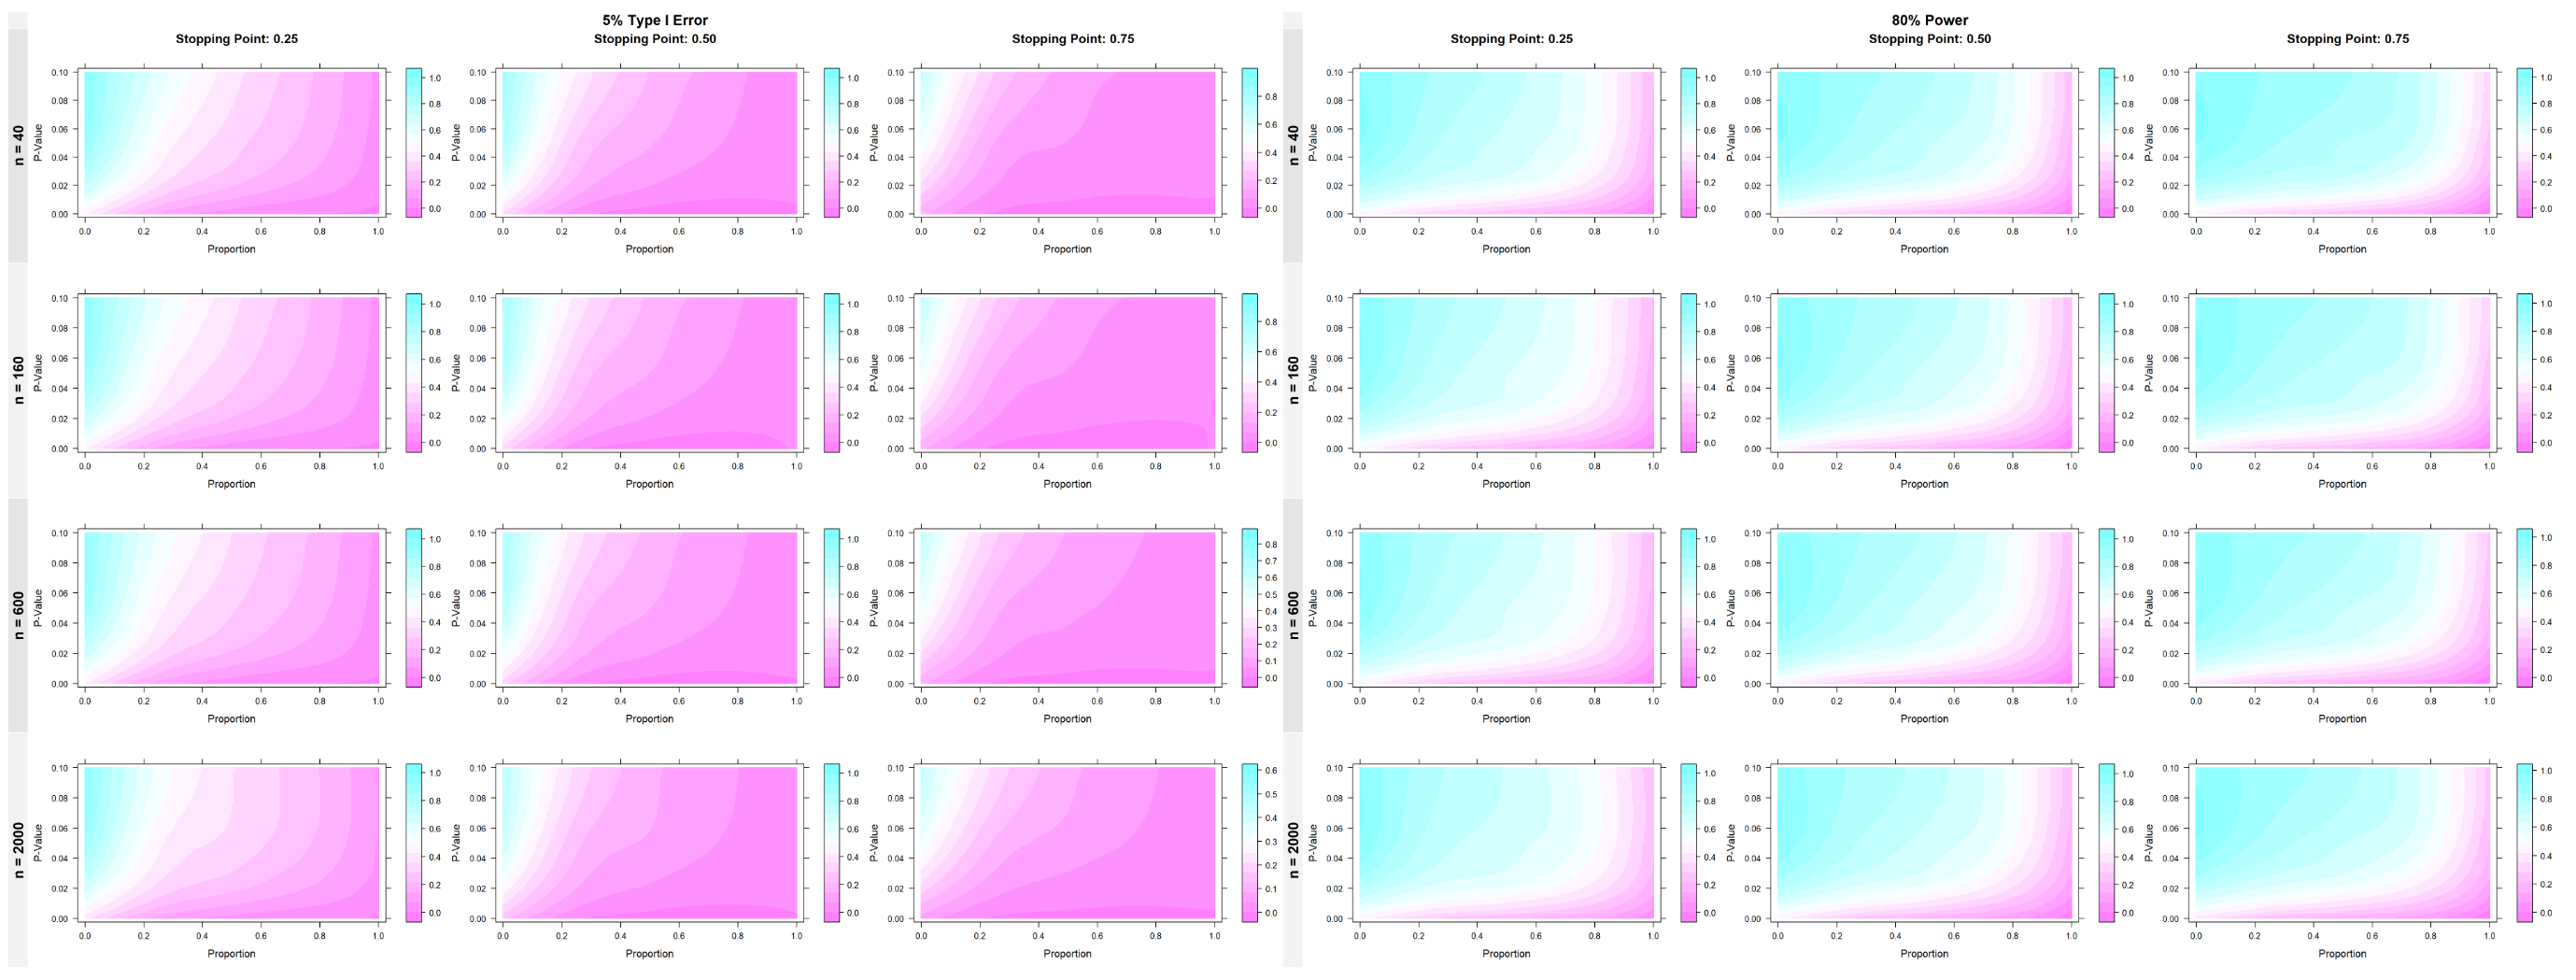
\includegraphics[width=\linewidth]{Fig1.png}
    \caption{Method Validation Results.  Likelihood of stopping shown for various threshold combinations and simulation settings}
    \label{fig:first}
  \end{minipage}\hfill%
\end{figure*}

\subsection{Method Calibration Results}

From the multiple calibration strategies considered, a single p value/proportion threshold combination was ultimately selected for each sample size and interim stopping point combination to optimize power while controlling type I error for efficacy monitoring (or level of significance and type II error for futility monitoring).  Out of the selected optimal thresholds, the variable calibration strategy performed best, with fixed p value and fixed proportion calibration strategies also performing well.  Strictly fixed p value and proportion calibration strategies performed slightly worse, which is unsurprising given these strategies are mush more restricted.  Arbitrary calibration performed tolerably well for certain stopping points and sample sizes, but was much less reliable and is not recommended for general use.  Variable calibration is recommended as the best and most flexible approach to selecting optimized threshold values, but fixing either the p value or proportion threshold and then calibrating the other is a simplified and still valid alternative calibration approach.

\subsection{Method Application Results}

\subsubsection{Futility Only Monitoring Results}

For simulations with a total sample size of 40, PO produced the lowest expected sample size followed by CU, AU, OBF, and GU.  For simulations with a total sample size of 160, CU produced the lowest expected sample size followed by PO, AU, OBF, and GU.  For simulations with a total sample size of 600, CU produced the lowest expected sample size followed by PO, GU, AU, and OBF (GU and AU however saw their rankings reverse for the 80\% and 95\% power scenarios).  For simulations with a total sample size of 2000, CU produced the lowest expected sample size followed by PO, GU, AU, and OBF.  Expected sample size tended to increase as power increased, indicating that all methods stopped later and less often for futility given higher power to detect a difference between treatment groups. 

For simulations with a total sample size of 40, the proportion of trials that rejected the null hypothesis at trial completion (without stopping early for futility) was highest using OBF, followed by GU, PO, AU, and CU (PO and GU however saw their rankings reversed for the 80\% and 95\% power scenarios).  For simulations with a total sample size of 160, the proportion of trials that rejected the null hypothesis at trial completion (without stopping early for futility) was highest using OBF, followed by GU, PO, AU, and CU (PO and AU however saw their rankings reversed for the 80\% and 95\% power scenarios).  For simulations with a total sample size of 600 and 2000, the proportion of trials that rejected the null hypothesis at trial completion (without stopping early for futility) was highest using OBF and lowest using CU.  GU, AU, and PO switched order frequently across power settings but remained relatively close in terms of absolute rejection rate.  For the null (5\% power) scenarios at all sample sizes, all methods produced rejection rates below 5\%, indicating that type I error was controlled.  The proportion of trials that rejected the null hypothesis tended to increase as power increased, indicating that all methods were more likely to reach the full sample size (without stopping early for futility) and then reject the null hypothesis given higher power to detect a difference between treatment groups.

For simulations with a total sample size of 40, the proportion of trials that stopped early for futility was highest using PO, followed by CU, GU, OBF, and AU (OBF and AU however saw their rankings reversed for the 80\% and 95\% power scenarios).  For simulations with a total sample size of 160, the proportion of trials that stopped early for futility was highest using CU, followed by PO.  OBF, AU, and GU switched order frequently across power settings but remained relatively close in terms of absolute early stopping rate.  For simulations with a total sample size of 600, the proportion of trials that stopped early for futility was highest using CU, followed by PO, GU, AU, and OBF (PO and GU switched rankings in the 5\% and 50\% power scenarios, while AU and OBF switched rankings in the 5\% power scenario).  For simulations with a total sample size of 2000, the proportion of trials that stopped early for futility was highest using CU, followed by GU, PO, AU, and OBF (GU and PO switched rankings in the 95\% power scenario, while AU and OBF switched rankings in the 5\% power scenario).  The proportion of trials that stopped early for futility tended to decrease as power increased, indicating that all methods were less likely to stop early for futility given higher power to detect a difference between treatment groups.

\subsubsection{Efficacy Only Monitoring Results}

For simulations with a total sample size of 40, AU produced the lowest expected sample size followed by GU, CU, PO, and OBF.  For simulations with a total sample size of 160, 600, and 2000, AU produced the lowest expected sample size followed by CU, GU, PO, and OBF.  Expected sample size tended to decrease as power increased, indicating that all methods stopped earlier and more often for efficacy given higher power to detect a difference between treatment groups.  The difference in expected sample size between upstrapping methods and group sequential methods was much more pronounced compared to futility only monitoring, with upstrapping methods consistently having lower expected sample size across all power and total sample size settings.  Additionally, when comparing among upstrapping methods the arbitrary calibration strategy consistently had the absolute lowest expected sample size of all methods considered.  This means that upstrapping methods are more likely to stop early for efficacy only monitoring regardless of sample size or power  

For simulations with a total sample size of 40, the proportion of trials that rejected the null hypothesis at trial completion or stopped early for efficacy was highest using AU, followed by GU, CU, OBF, and PO (GU and CU however saw their rankings reversed for the 95\% power scenario).  For simulations with a total sample size of 160 or 2000, the proportion of trials that rejected the null hypothesis at trial completion or stopped early for efficacy was highest using AU, followed by CU, GU, OBF, and PO.  For simulations with a total sample size of 600, the proportion of trials that rejected the null hypothesis at trial completion or stopped early for efficacy was highest using AU, followed by CU, GU, OBF, and PO (AU and CU however saw their rankings reverse for the 95\% power scenario, while OBF and PO reversed rankings for the 5\% power scenario).  For the null (5\% power) scenarios at all sample sizes, group sequential methods produced rejection rates below 5\%, indicating that type I error was controlled.  Upstrapping methods however, consistently produced rejection rates well above the 5\% target for type I error, indicating that type I error rate was not successfully controlled.  The proportion of trials that rejected the null hypothesis tended to increase as power increased, indicating that all methods were more likely to either stop early for efficacy or reach the full sample size and then reject the null hypothesis given higher power to detect a difference between treatment groups.  These results show that upstrapping methods (AU in particular) are more likely to stop early or reject the null hypothesis using the full dataset during efficacy only monitoring, which is consistent with the expected sample size results above.

For simulations with a total sample size of 40, the proportion of trials that stopped early for efficacy was highest using AU, followed by GU, CU, PO, and OBF (GU and CU however saw their rankings reversed for the 95\% power scenario).  For simulations with a total sample size of 160, the proportion of trials that stopped early for efficacy was highest using AU, followed by CU, GU, PO, and OBF (AU and CU however saw their rankings reversed for the 95\% power scenario).  For simulations with a total sample size of 600 and 2000, the proportion of trials that stopped early for efficacy was highest using AU, followed by CU, GU, PO, and OBF (AU, CU, and GU switched rankings in the 95\% power scenario).  The proportion of trials that stopped early for efficacy tended to increase as power increased, indicating that all methods were more likely to stop early for efficacy given higher power to detect a difference between treatment groups.  As seen in the expected sample size and rejection rate results, upstrapping methods were more aggressive in stopping early for efficacy, especially when using arbitrary calibration.

\begin{figure*}[t]
  \begin{minipage}[t]{1\linewidth}
    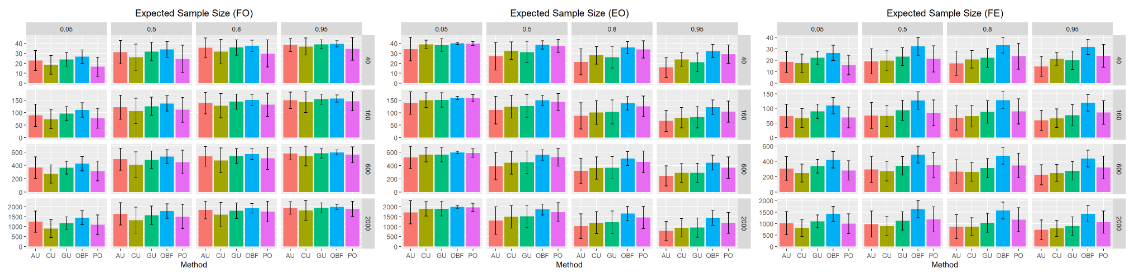
\includegraphics[width=\linewidth]{Fig2.png}
    \caption{Expected Sample Size Results}
    \label{fig:second}
  \end{minipage}\hfill%
\end{figure*}
\begin{figure*}[t]
  \begin{minipage}[t]{1\linewidth}
    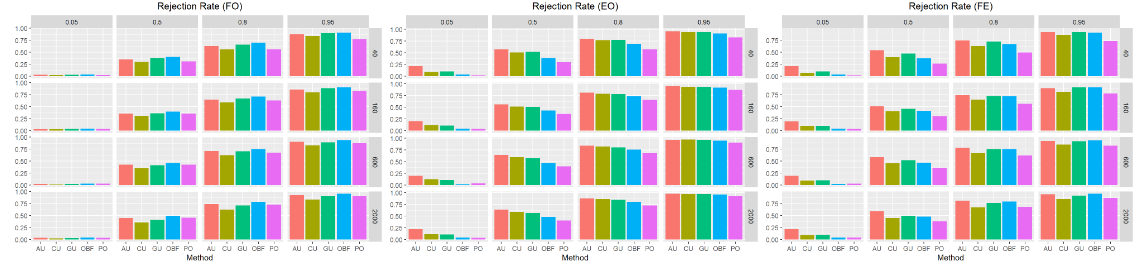
\includegraphics[width=\linewidth]{Fig3.png}
    \caption{Rejection Rate Results}
    \label{fig:third}
  \end{minipage}\hfill%
\end{figure*}
\begin{figure*}[t]
  \begin{minipage}[t]{1\linewidth}
    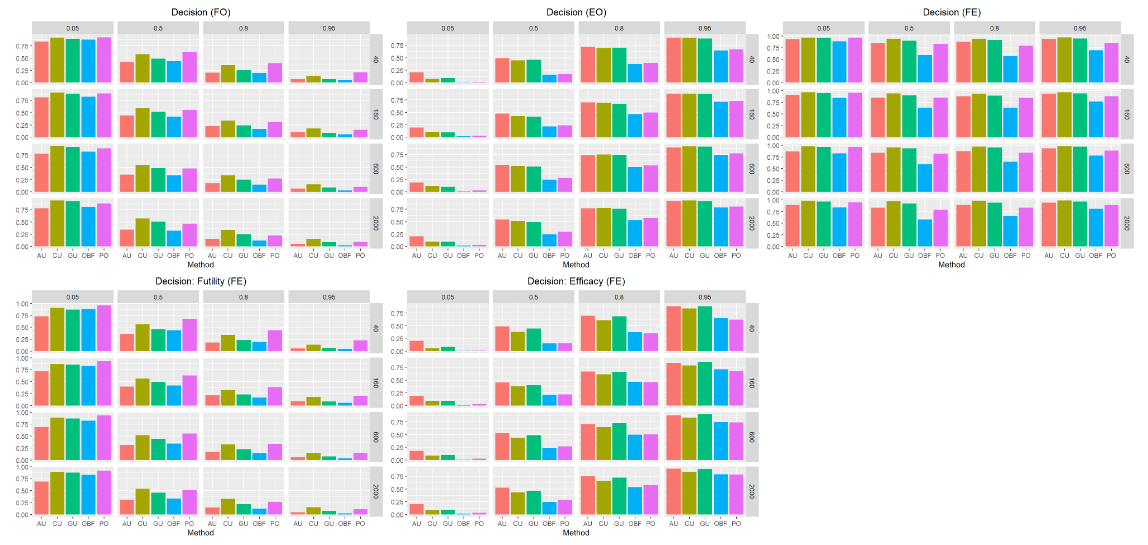
\includegraphics[width=\linewidth]{Fig4.png}
    \caption{Interim Stopping Decision Results}
    \label{fig:fourth}
  \end{minipage}\hfill%
\end{figure*}

\subsubsection{Futility/Efficacy Monitoring Results}

For simulations across all total sample sizes, OBF produced the highest expected sample size while GU, AU, CU, and PO switched order frequently across power settings.  Overall, expected sample size showed a less clear trend when interim monitoring is performed simultaneously for futility and efficacy.  For all methods, expected sample size tended to increase and then decrease as power increased, indicating that the combination of efficacy and futility monitoring are stopping more often on average when the power to detect a significant difference between treatment groups is either very high (efficacy) or very low (futility).  

For simulations with a total sample size of 40, the proportion of trials that rejected the null hypothesis at trial completion (without stopping early for futility) or stopped early for efficacy was highest using AU, followed by GU, CU, OBF, and PO (CU and OBF however saw their rankings reversed for the 80\% and 95\% power scenarios).  For simulations with a total sample size of 160, the proportion of trials that rejected the null hypothesis at trial completion (without stopping early for futility) or stopped early for efficacy was lowest using PO, while OBF, CU, GU, and AU switched order frequently across power settings.  For simulations with a total sample size of 600 or 2000, the proportion of trials that rejected the null hypothesis at trial completion (without stopping early for futility) or stopped early for efficacy was not consistently highest or lowest for a single method.  For the null (5\% power) scenarios at all sample sizes, group sequential methods produced rejection rates below 5\%, indicating that type I error was controlled.  Upstrapping methods however, consistently produced rejection rates well above the 5\% target for type I error, indicating that the type I error rate was not successfully controlled.  The proportion of trials that rejected the null hypothesis (without stopping for futility) or stopped early for efficacy tended to increase as power increased, indicating that all methods were more likely to either stop early for efficacy or reach the full sample size and then reject the null hypothesis given higher power to detect a difference between treatment groups.
For simulations with any given total sample size, the proportion of trials that stopped early for either futility or efficacy was highest using CU, followed by GU, AU, PO, and OBF (GU, AU, and PO however saw their rankings switched for the 5\% power scenario).  Similarly to the efficacy only results, this shows that upstrapping methods are more likely to stop early.  The proportion of trials that stopped early tended to decrease and then increase as power increased, indicating that the combination of efficacy and futility monitoring are more likely to stop early when the power to detect a significant difference between treatment groups is either very high (efficacy) or very low (futility).

For simulations with a total sample size of 40 and 160, the proportion of trials that stopped early specifically for futility was highest using PO, followed by CU (OBF, GU, and AU however saw their rankings switched for all power scenarios).  For simulations with a total sample size of 600, the proportion of trials that stopped early specifically for futility was highest using PO, followed by CU, GU, OBF, and AU (OBF and AU however saw their rankings reversed in the 80\% and 95\% power scenarios).  For simulations with a total sample size of 2000, the proportion of trials that stopped early specifically for futility was not consistently highest or lowest for a single method.  The proportion of trials that stopped early specifically for futility tended to decrease as power increased, indicating that all methods were less likely to stop early for futility given higher power to detect a difference between treatment groups.

For simulations with a total sample size of 40, the proportion of trials that stopped early specifically for efficacy was highest using AU, followed by GU, CU, PO, and OBF (PO and OBF however saw their rankings reversed for the 80\% and 95\% power scenarios).  For simulations with a total sample size of 160 and 600, the proportion of trials that stopped early specifically for efficacy was not consistently highest or lowest for a single method.  For simulations with a total sample size of 2000, the proportion of trials that stopped early specifically for efficacy was highest using AU, followed by GU, CU, PO, and OBF (PO and OBF however saw their rankings reversed for the 95\% power scenario).  The proportion of trials that stopped early specifically for efficacy tended to increase as power increased, indicating that all methods were more likely to stop early for efficacy given higher power to detect a difference between treatment groups.

\section{Discussion}

\subsection{Limitations}

This research is meant primarily as an explorative study of whether upstrapping is a reasonable approach for interim monitoring.  Accordingly, many simplifying assumptions were made at both the simulation and modeling stages of analysis.  We considered simulation settings based only on sample size, interim stopping point, and power.  All simulations assumed uniform subject accrual over time, and a constant treatment efficacy rate.  To further test performance of the upstrap algorithm more complex simulations that account for time varying trends in disease condition over time will be necessary.  It may also be worth considering more complicated modeling strategies (potentially with covariate information included) that more closely mirror common clinical trial settings in practice.

Calibration and application results showed a clear trade off between power and type I error rate for the upstrapping method, particularly when efficacy monitoring is needed.  This is not unexpected, but is an important consideration when deciding on an interim monitoring method and choosing threshold values.  Another potential extension to this research would be to define a novel spending function to optimize this trade off and make adjustments for multiple stopping points over the course of the trial to control the overall type I error rate, similar to group sequential methods but specifically designed for upstrapping.  In general, we considered several different approaches to threshold calibration and chose the best values based on power and type I error rate (or level of significance and type II error rate for futility monitoring) considerations.  However, this process could easily be extended to consider a wider variety of approaches or a more granular grid of potential threshold values.

\subsection{Conclusions}

Based on the validation results of upstrapped futility monitoring in both null and alternative settings, we can conclude that applying the algorithm in this context appears to produce reasonable results, as long as calibration is performed beforehand to select appropriate p value and proportion thresholds to define trial success.  This holds true across a wide variety of sample sizes and interim stopping points, and comparing results between differing power scenarios indicates that the algorithm is able to successfully return higher likelihood of stopping for futility under the null case (power = 5\%) compared to the alternative case (power = 80\%).

While there are many nuanced approaches to calibrating the p value and proportion thresholds, we recommend using simulated data to select optimal thresholds based on the appropriate power and type I error rate (or level of significance and type II error rate for futility monitoring), preferably without setting restrictions on the potential combinations of p value and proportion thresholds.  While arbitrary calibration is able to achieve success in certain limited cases, it did not prove sufficient in most cases; with performance being particularly low for efficacy monitoring and in trials with small sample sizes.  Using O’Brien-Fleming inspired p value thresholds does not appear to yield significantly superior outcomes overall, and is therefore not considered necessary based on these results.

For the futility only monitoring case, the AU, CU, and GU methods all perform similarly well when compared to OBF and PO across a variety of power and total sample size settings.  This means that when trials are designed with the option to stop early for futility but not efficacy, upstrapping can be used reliably based on expected sample size, trial rejection rate, and early stopping rate.  For the efficacy only monitoring case across a variety of power and total sample size settings, the AU, CU, and GU methods all saw lower expected sample size when compared to OBF and PO and were much more likely to stop early for efficacy and/or reject the null hypothesis at trial conclusion.  Based on the null scenario results however, upstrapping methods did not perform well in terms of controlling type I error rate.  This means that when trials are designed with the option to stop early for efficacy but not futility, the choice to use upstrapping or group sequential designs will depend on the tradeoff between lower expected sample size with higher power vs higher type I error.  For the dual futility and efficacy monitoring case, it was more difficult to extract clear trends in expected sample size, rejection rate, and early stopping rate across the various power and total sample size settings.  Based on the null scenario results however, upstrapping methods consistently performed poorly with regards to controlling type I error rate.  This means that when trials are designed with the option to stop early for either futility or efficacy, upstrapping is not likely to be desirable based on expected sample size, trial rejection rate, or early stopping rate.

%%%%%%%%%%%%%%%%%%%%%%%%%%%%%%%%%%%%%%%%%%%%%%%%%%%%%%%% References
\begin{thebibliography}{99}
\bibitem[1]{R1}
DeMets, D. L., \& Lan, K. K. (1994). Interim analysis: the alpha spending function approach. \textit{Statistics in medicine, 13}(13-14), 1341–1356. https://doi.org/10.1002/sim.4780131308

\bibitem[2]{R2}
K.K. Gordon Lan, David M. Reboussin \& David L. DeMets (1994) Information and information fractions for design and sequential monitoring of clinical trials, Communications in Statistics - Theory and Methods, 23:2, 403-420, DOI: 10.1080/03610929408831263

\bibitem[3]{R3}
Jennison, C. and Turnbull, B. W. (1999). Group sequential methods with applications to
clinical trials. CRC Press

\bibitem[4]{R4}
Kaizer, A. M., Wild, J., Lindsell, C. J., Rice, T. W., Self, W. H., Brown, S., Thompson, B. T., Hart, K. W., Smith, C., Pulia, M. S., Shapiro, N. I., \& Ginde, A. A. (2022). Trial of Early Antiviral Therapies during Non-hospitalized Outpatient Window (TREAT NOW) for COVID-19: a summary of the protocol and analysis plan for a decentralized randomized controlled trial. \textit{Trials, 23}(1), 273. https://doi.org/10.1186/s13063-022-06213-z

\bibitem[5]{R5}
O'Brien, P. C., \& Fleming, T. R. (1979). A multiple testing procedure for clinical trials. \textit{Biometrics, 35}(3), 549–556.

\bibitem[6]{R6}
Pocock, S. J. (1977). Group Sequential Methods in the Design and Analysis of Clinical Trials. \textit{Biometrika, 64}(2), 191–199. https://doi.org/10.2307/2335684

\bibitem[7]{R7}
Crainiceanu, C. M., \& Crainiceanu, A. (2020). The upstrap. \textit{Biostatistics (Oxford, England), 21}(2), e164–e166. https://doi.org/10.1093/biostatistics/kxy054

\bibitem[8]{R8}
Alsouqi, A., Deger, S. M., Sahinoz, M., Mambungu, C., Clagett, A. R., Bian, A., Guide, A., Stewart, T. G., Pike, M., Robinson-Cohen, C., Crescenzi, R., Madhur, M. S., Harrison, D. G., \& Ikizler, T. A. (2022). Tissue Sodium in Patients With Early Stage Hypertension: A Randomized Controlled Trial. \textit{Journal of the American Heart Association, 11}(8), e022723. https://doi.org/10.1161/JAHA.121.022723

\end{thebibliography}

\end{document}